\section{Methods}
\label{sec:methods}

\subsection{Dataset}
\label{subsec:dataset}
The prostate and the peripheral zone (PZ) were manually
contoured on T2-weighted Axial MRI (T2W) in MIM (MIM Software Inc,
Cleveland, OH, USA) by imaging experts (RS, ALB) with more than
25 years combined expertise in prostate cancer. The contours were cross
checked by the two imaging experts and reviewed by radiation
oncologists (MCA, AP) with extensive expertise in genitourinary
malignancies. Two datasets were considered: (i) imaging data from the
SPIE-AAPM-NCI PROSTATEx Challenge \cite{deukwoo_classification_2018} (328 cases), 
acquired on two different types of Siemens 3T MR scanners, the MAGNETOM Trio
and Skyra (Siemens, Erlangen, Germany), and  (ii) MRI data from
patients in radiotherapy clinical trials at the University of Miami (100 cases),
acquired on Discovery MR750 3T MRI (GE, Waukesha, WI, USA).


\subsection{Preprocessing}
\label{subsec:prepro}
The proposed preprocessing steps for the MRIs consist of: bias correction using the N4ITK algorithm \cite{n4itk}, image normalization to an interval of [0,1], automatic selection of a region of interest (ROI), image re-sampling to a resolution of $0.5 \times 0.5 \times 0.5$ mm, and contour interpolation using optical flow.  

The method for selecting the ROI was originally proposed in \cite{anneke}. It consists of reducing the size of the MRIs (axial, sagittal, and coronal) by cropping the images with the volume that comes from the intersection of the rectangular prisms for the three planes. Resampling is performed using linear interpolation and is programmed with the ITK software \cite{itk}.  Figure \ref{fig_1} shows an example of the resulting image after being preprocessed with bias correction, normalization, and cropped to a ROI. 

%\begin{figure}[h]
%    \centering
%    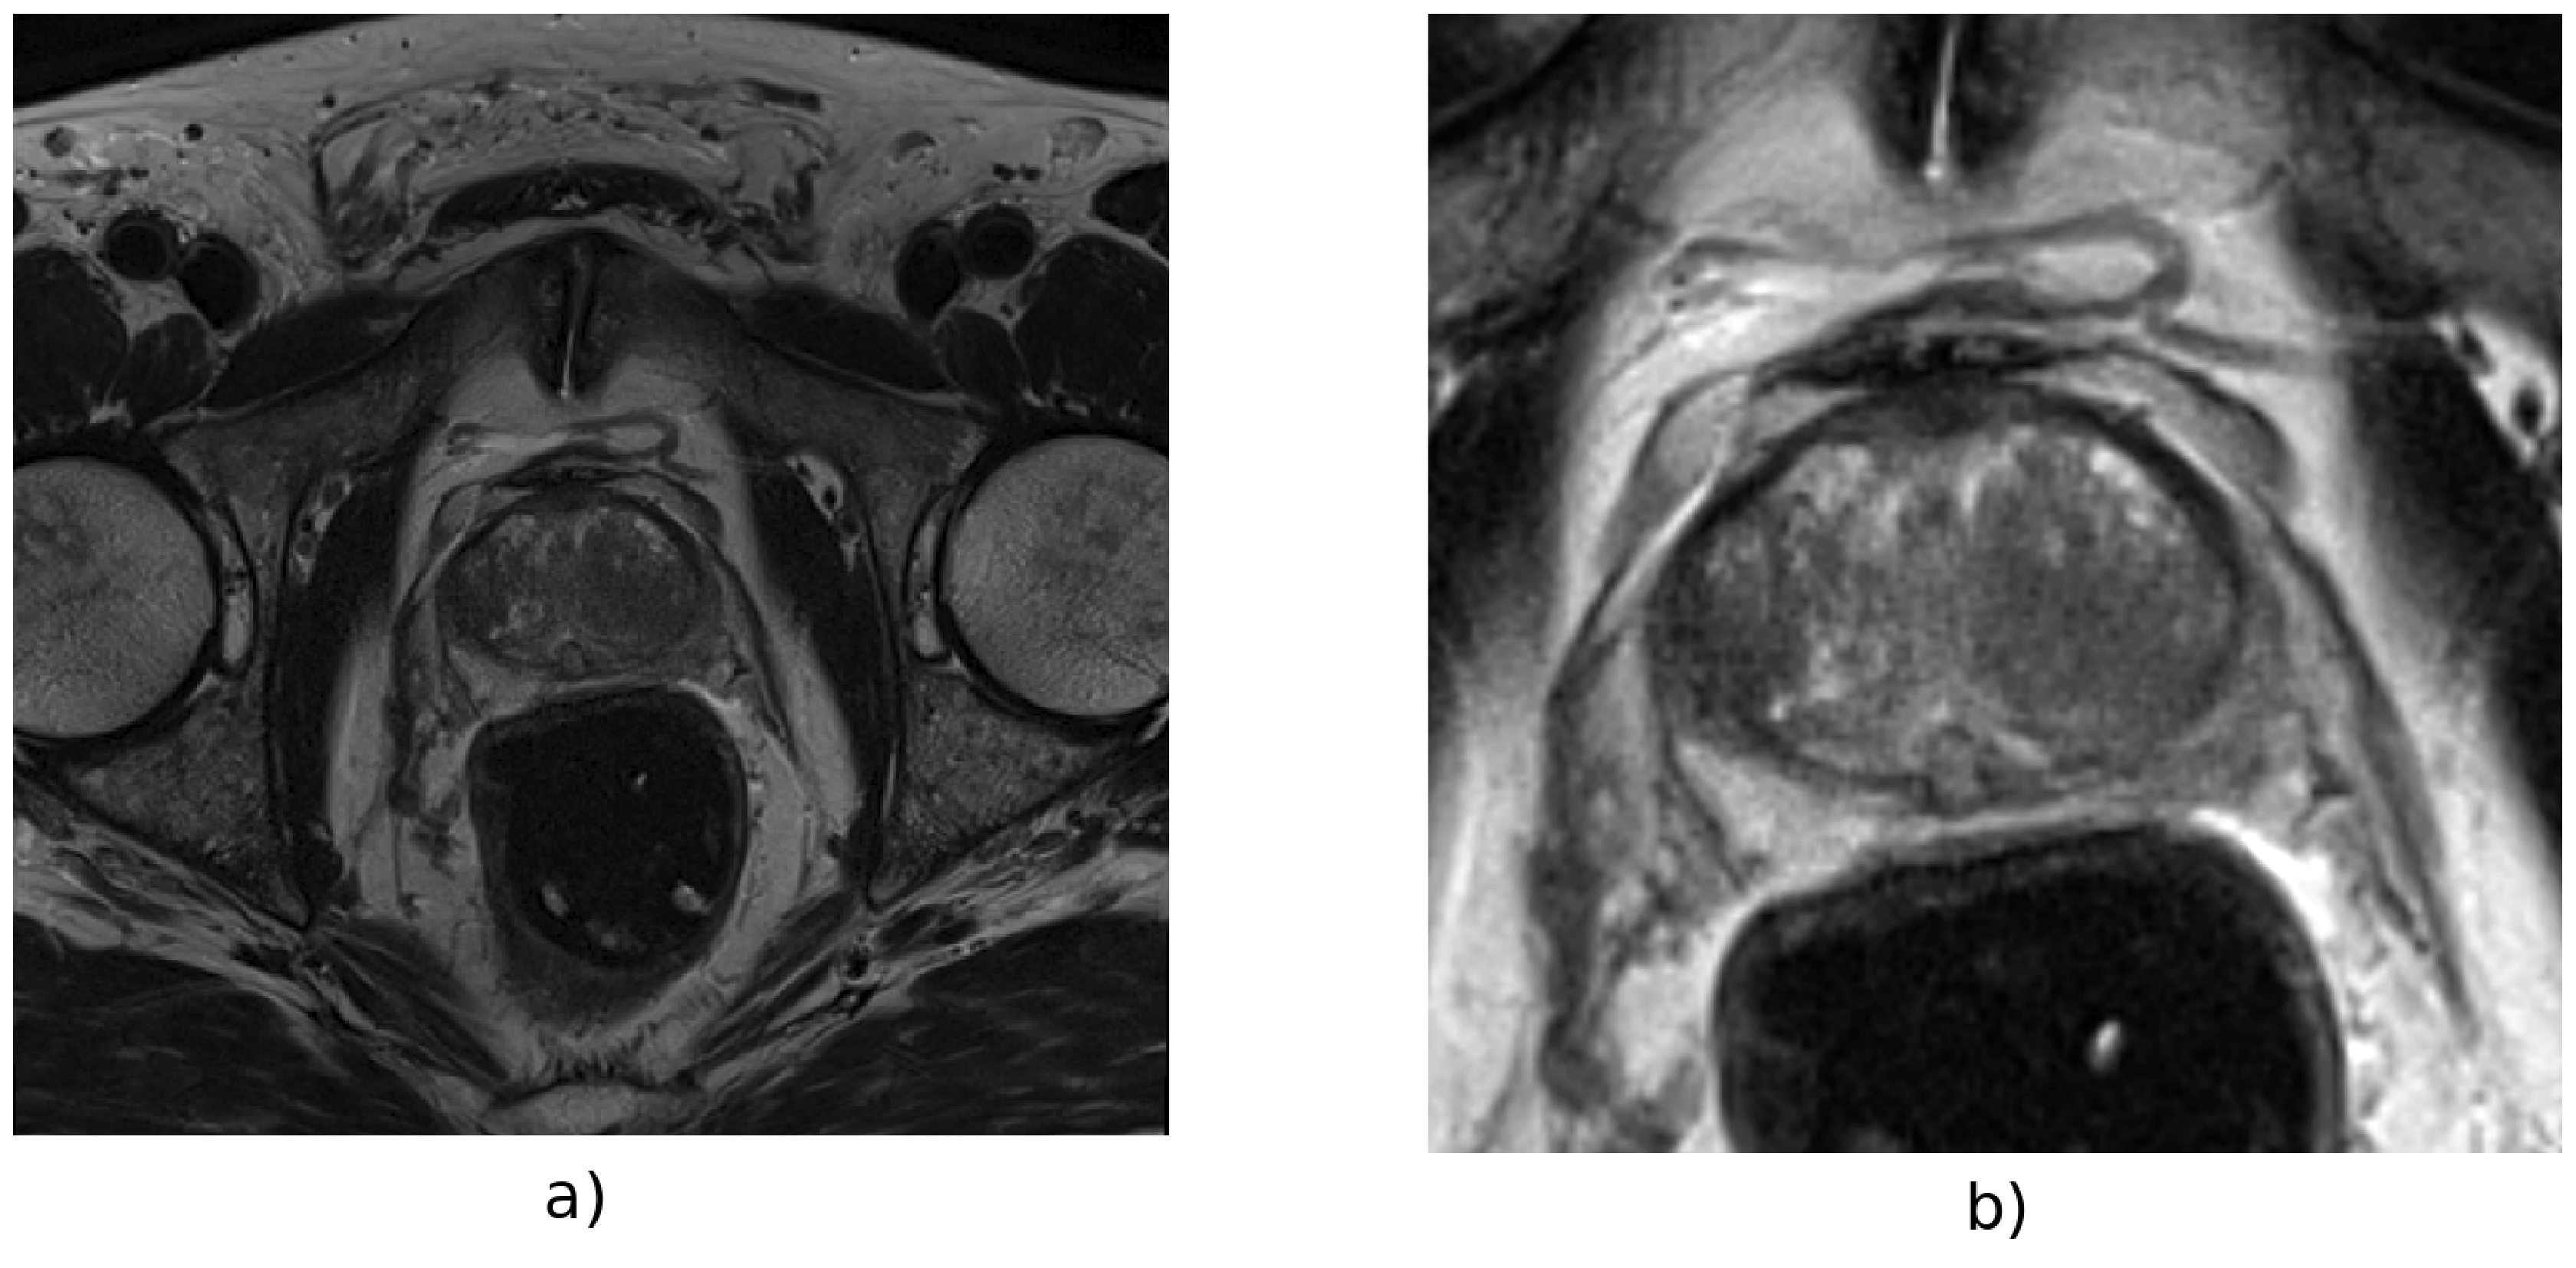
\includegraphics[totalheight=.25\textheight]{figures/Figure1.eps}
%    \caption{The MRIs are preprocessed with bias correction, normalization, resampling, and cropped to a ROI to reduce the variability of sizes and intensities between magnets. In this example, \textbf{a)} is the original image and \textbf{b)} is the image after being processed.} 
%    \label{fig_1}
%\end{figure}

Manual contours made by the experts were carried on the original MRI resolutions and not on the higher resolution version; therefore, the necessity for interpolating them.  The proposed interpolation is performed in two dimensions and is computed independently between every two consecutive horizontal slices. First, optical flow is obtained between the two contours using the Farneback method \cite{optflow}. Then, the contours are interpolated linearly following the direction of the optical flow. Figure \ref{fig:fig_2} shows an example of the optical flow obtained between two horizontal slices and the resulting interpolated contour using this method. 

%\begin{figure}[h]
%    \centering
%    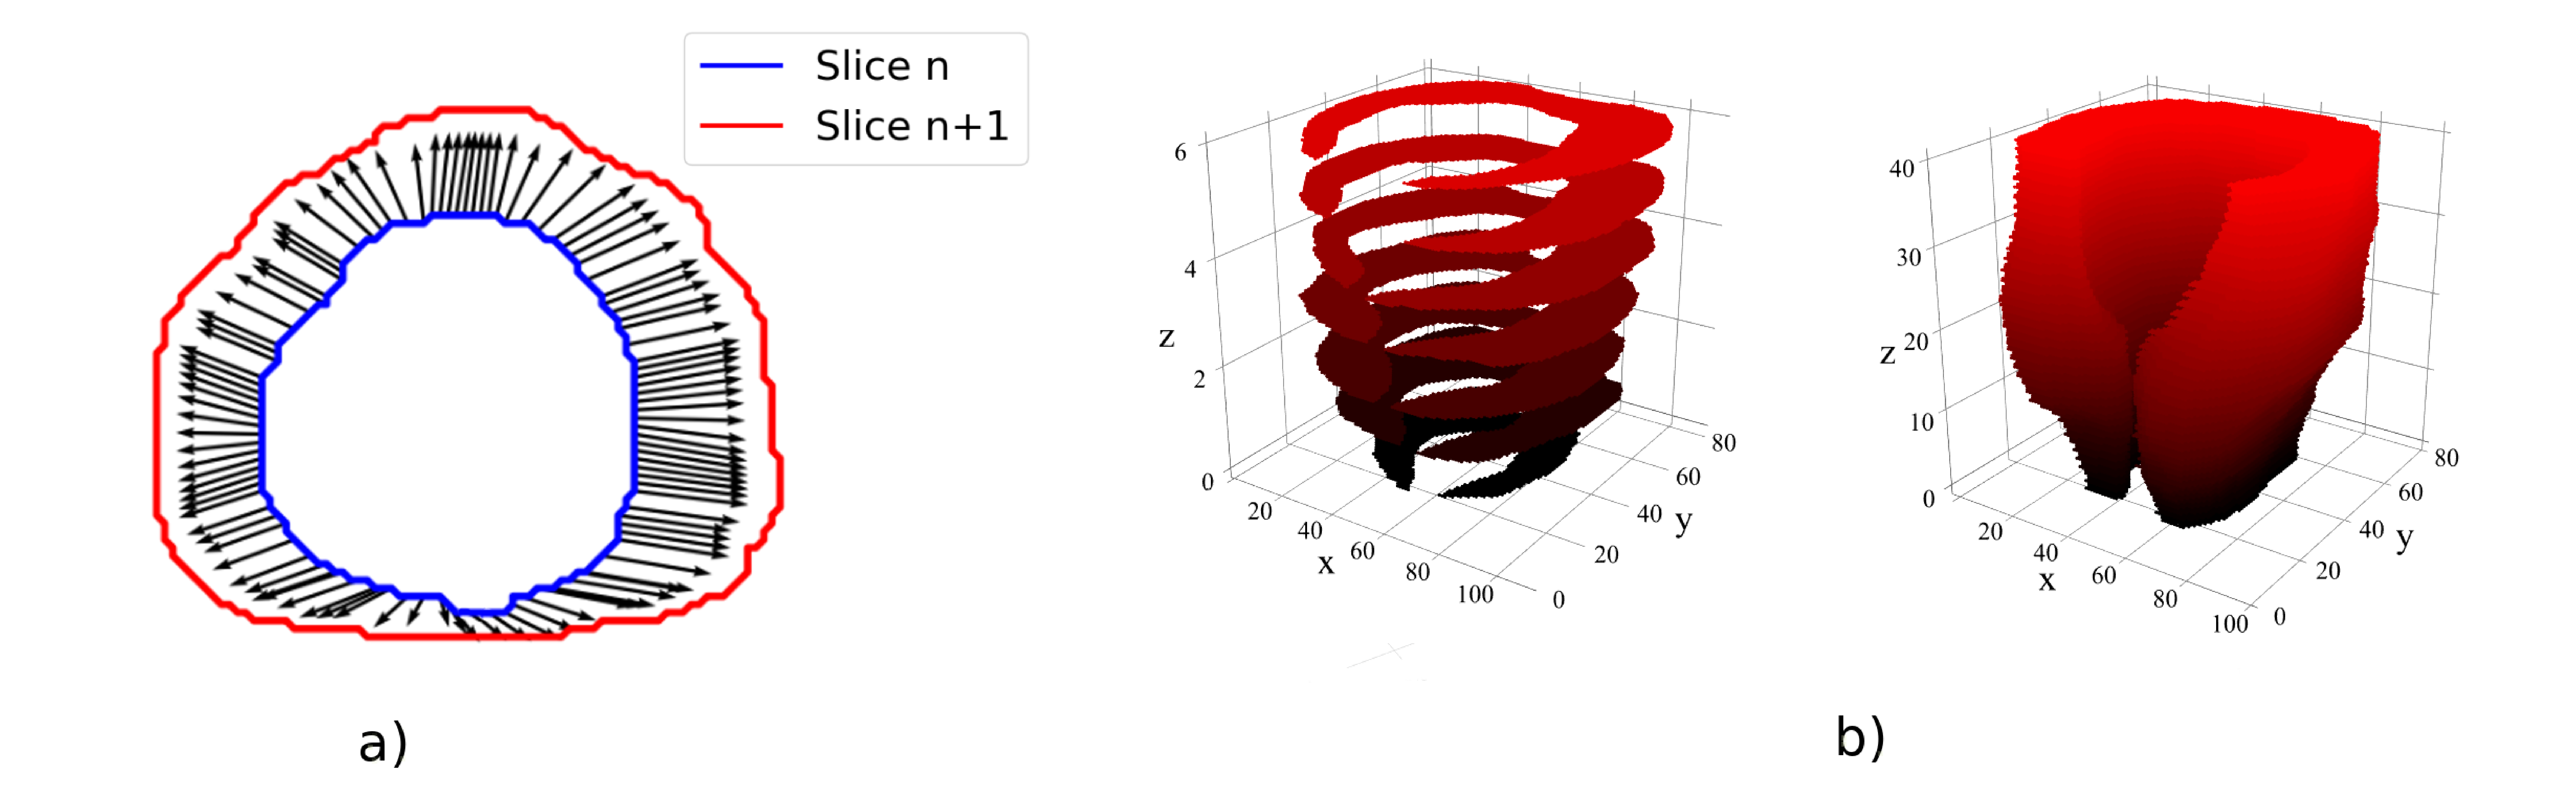
\includegraphics[totalheight=.21\textheight]{figures/Figure2.eps}
%    \caption{Example of the proposed algorithm to increase the resolution of prostate and PZ contours. In \textbf{a)}, an example of the optical flow obtained between two prostate contours from adjacent horizontal planes. In \textbf{b)} on the left, original contours with 17 slices. On the right, interpolated contours with 68 slices.}
%    \label{fig:fig_2}
%\end{figure}



\subsection{3D-CNN architecture}
The proposed CNN consist of a 3D multistream architecture that follows the analysis and synthesis path of the 3D U-Net \cite{cciccek20163d}. Our implementation follows the one described by Anneke et al. in 2018  \cite{anneke}. The input of each stream is the post-processed ROI with a resolution of $168^3$ for one of three MRI series (axial, sagittal, and coronal). During the analysis phase, a group of two convolutional layers and one max pool layer is repeated three times. The second convolutional layer in each group doubles the number of filters.  In the synthesis phase, a similar set of two convolutional layers and one deconvolution is applied three times. We modified the original network by implementing batch normalization \cite{ioffe2015batch} and Dropout of 20\%  \cite{hinton2012improving} after each convolution in the synthesis path.\\

We also cut down on the number of filters from $192$ to $28$ in the largest convolutional layer (after the first concatenation) reducing the number of parameters from to 995k to 663k. These changes cut the training time in half and improved the generalization of the  model. Figure \ref{fig:fig_3} shows the proposed model; all convolutional layers use a filter size of $3 \times 3 \times 3$ and rectified linear unit (ReLu) as the activation function; except the last layer which uses a filter size of $1 \times 1 \times 1$ and Sigmoid as the activation function to match the resolution of the input MRI series.
% fig:fig_3

\subsection{Training}
\label{subsec:training}
The selected optimization algorithm is Stochastic Gradient Descent (SGD) with a learning rate $\alpha = 0.001$, momentum of 0.9 and decay of $10^{-6}$. The training is performed for 1000 epochs with an early stop mechanism if the loss function is not improved by at least $\delta = 0.001$ after 70 iterations. The Loss function used is the negative Dice Similarity Coefficient (DSC) \cite{dice1945measures}:  
\begin{equation}
\text{Loss} = - \frac{2 \sum_{i=1}^{N}p_it_i}{\sum_{i=1}^{N}p_i^2 + \sum_{i=1}^{N}t_i^2 + \varepsilon} 
\label{eq:dsc}
\end{equation}
where N is the total number of voxels in the image, $p_i$ the voxel values for the prediction of the network, $t_i$ the true voxel values of the prostate or PZ masks, and $\varepsilon = 1$ for all the models.

In order to compare the robustness of the models with respect to changes in MRI vendor machines,  a distinct model was trained for each dataset: GE (n=220), Siemens (n=330), and combined model (n=550). Each dataset was split into 90\% for training and 10\% for validation. Data augmentation was performed on the fly by flipping the images in the sagittal axis and blurring them using 3D Gaussian blur randomly with $0 \leq \sigma \leq 3$. Each data augmentation method is applied with a random chance of $1/2$.  
A total number of six models are compared, three for the prostate been trained with each dataset and three more for the PZ. 

The training was performed on a desktop computer with an Intel Xeon(R) E5-2609 CPU and a GeForce GTX 1080 Ti NVIDIA GPU. The system is implemented using Keras \cite{chollet2015} and Tensor Flow \cite{tensorflow2015-whitepaper} python libraries. The average training time for each model, independently if its for the prostate or the PZ, is $\sim 7.5$ hours, the overall training time for the six models is about two days.

\subsection{Postprocessing}
The CNN outputs a 3D volume of the same size of the ROI, in our case $168^3$, and each voxel gets the probability of belonging to the area of interest (prostate or PZ) versus the background. From this volume a binary mask is obtained with a threshold value of 0.5. After that, the largest connected volume is selected. Finally, the 3D DSC for the contour of interest in the resampled image and in the original MRI series resolution is computed. The prediction of the PZ contour is intersected with the prostate, restricting it to the prostate volume.